\documentclass{article}
\usepackage[utf8]{inputenc}
\usepackage[english]{babel}
\usepackage[]{amsthm} 
\usepackage[]{amssymb} 
\usepackage{amsmath}
\usepackage{graphicx}
\graphicspath{ {./prob1_img/} }
\usepackage{hyperref}
\usepackage{mathtools}
\usepackage[thinc]{esdiff}
\usepackage[dvipsnames]{xcolor}
\usepackage{float}
\newtheorem*{theorem}{Theorem}

\title{ADSP: HW1}
\author{Lo Chun, Chou \\ R13922136}
\date\today


\begin{document}
\setlength{\parindent}{0pt}
\maketitle 

\section*{(1)}

\subsection*{(a)}

\begin{figure}[h]
    \centering
    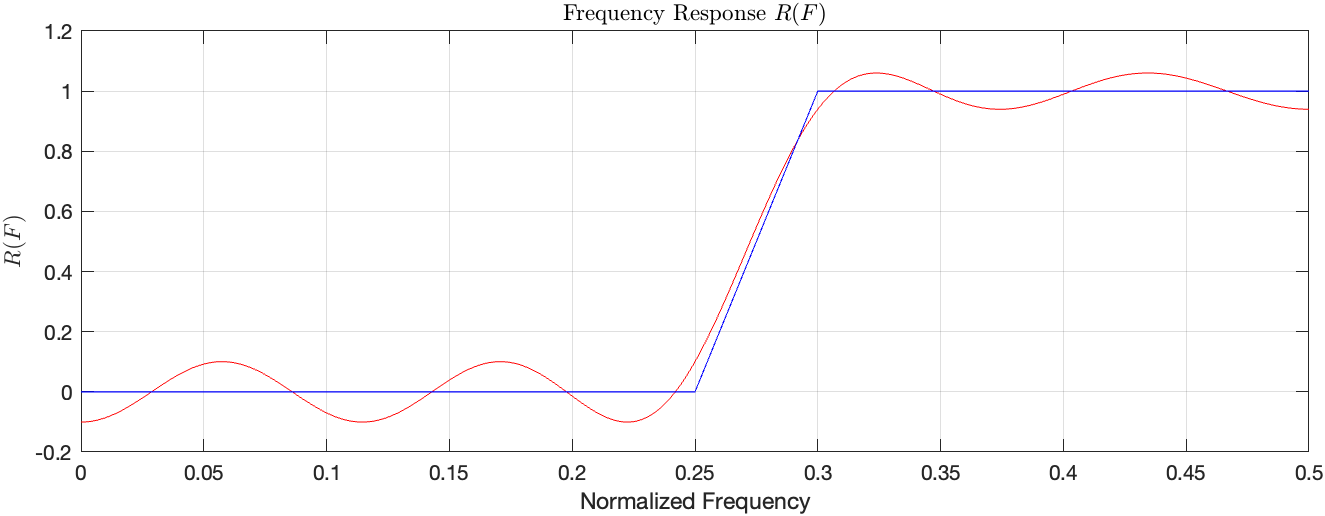
\includegraphics[width=0.7\textwidth]{frequency_response}
\end{figure}

\subsection*{(b)}

\begin{figure}[h]
    \centering
    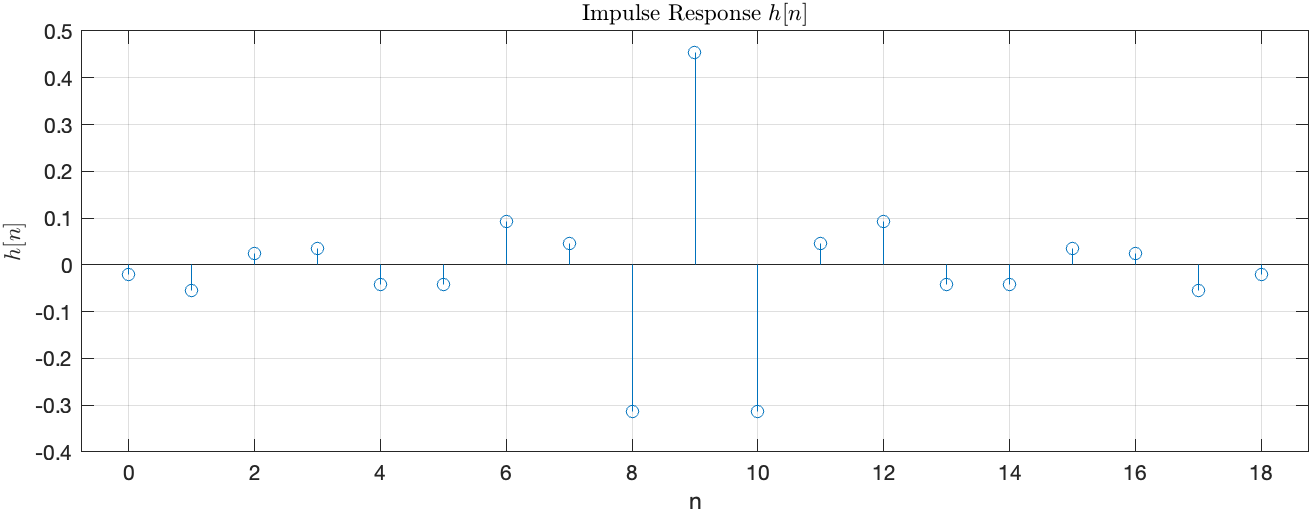
\includegraphics[width=0.7\textwidth]{impulse_response}
\end{figure}

\subsection*{(c)}
\begin{figure}[!htb]
    \centering
    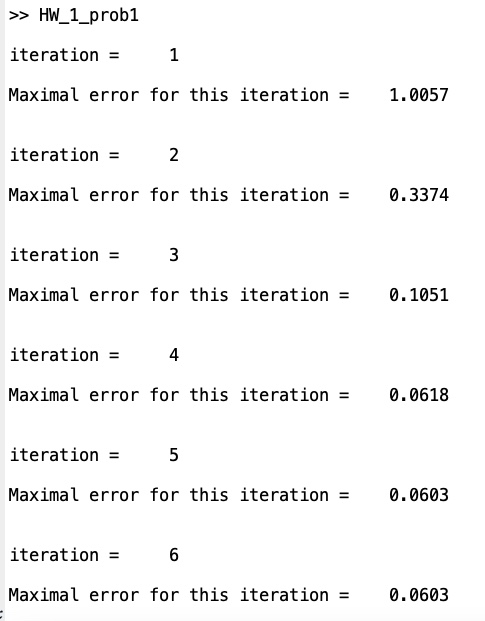
\includegraphics[width=0.7\textwidth]{maximal_error_this_iteration}
\end{figure}

\clearpage

\section*{(2)}

\subsection*{(a)}   

Originally, we have the convolution:

\begin{equation*}
    y[n] = x[n] * h[n]
\end{equation*}

By uising FT, we can transform this equation into:

\begin{equation*}
    Y(f) = X(f)H(f)
\end{equation*}

then taking $\log$ on both sides, we get:

\begin{equation*}
    \log Y(f) = \log X(f) + \log H(f)
\end{equation*}

\subsection*{(b)}

\begin{enumerate}
    \item We can use FT to do spectral analysis.
    \item We can use FT to convert convolution into multiplication.
\end{enumerate}

\subsection*{(c)}

\begin{enumerate}
    \item It is not a real operation, and we need to deal with irrational numbers, so the computation complexity is high.
    \item If the sampling frequency is too low (i.e. $f_s < 2B$), then aliasing will occur. (And if we try to prevent this to happen by increasing $f_s$, then more computation is needed.)
\end{enumerate}

\section*{(3)}

We have the given equations:

\begin{align*}
    y[n] &= x[n] * h[n] \\
    h[n] &= (0.7^n + (-0.6)^{n+1})u[n]  \quad \text{ where } u[n]: \text{ unit step function}
\end{align*}

We can first find $H(z)$ used in the $z$-transform:

\begin{align*}
    H(z) &= \sum_{n=-\infty}^{\infty} h[n]z^{-n} \\
    &= \sum_{n=-\infty}^{\infty} (0.7^n + (-0.6)^{n+1})u[n]z^{-n} \\
    &= \sum_{n=0}^{\infty} (0.7^n + (-0.6)^{n+1})z^{-n} \\
    &= \sum_{n=0}^{\infty} 0.7^nz^{-n} + \sum_{n=0}^{\infty} (-0.6)^{n+1}z^{-n} \\
    &= \sum_{n=0}^{\infty} (0.7 z^{-1})^n + (-0.6)\sum_{n=0}^{\infty} (-0.6 z^{-1})^n \\
    &= \frac{1}{1-0.7z^{-1}} + \frac{-0.6}{1-(-0.6z^{-1})} \\
    &= \frac{1}{1-0.7z^{-1}} - \frac{0.6}{1+0.6z^{-1}} \\
    &= \frac{(1+0.6z^{-1}) - (0.6 - 0.42z^{-1})}{(1-0.7z^{-1})(1+0.6z^{-1})} \\
    &= \frac{0.4 + 1.02z^{-1}}{(1-0.7z^{-1})(1+0.6z^{-1})} \\
\end{align*}

Since $Y(z) = H(z)X(z)$, by plugging in this result, and using the inverse $z$-transform, we get:

\begin{align*}
    &Y(z) = \frac{0.4 + 1.02z^{-1}}{(1-0.7z^{-1})(1+0.6z^{-1})}X(z) \\
    \Rightarrow \ &(1-0.7z^{-1})(1+0.6z^{-1})Y(z) = (0.4 + 1.02z^{-1})X(z) \\
    \Rightarrow \ & (1 - 0.1z^{-1} - 0.42z^{-2})Y(z) = (0.4 + 1.02z^{-1})X(z) \\
    \Rightarrow \ & Y(z) = (0.1z^{-1})Y(z) + (0.42z^{-2})Y(z) + 0.4X(z) + 1.02z^{-1}X(z) \\
    \Rightarrow \ &y[n] = 0.1y[n-1] + 0.42y[n-2] + 0.4x[n] + 1.02x[n-1] \qquad 
\end{align*}

\section*{(4)}

\subsection*{(a)}

We can use the step invariance method to reduce the aliasing effect because we take the integral of $h_a(t)$.
From the equation:

\begin{equation*}
    H_{a,u}(f) = \frac{H_a(f)}{j2\pi f}
\end{equation*}

we can see that when $f$ is large, the denominator is large, so the high-frequency part is decreased.

\subsection*{(b)}

The bilinear transform can fully avoid the aliasing effect because 
by converting the original frequency to the new frequency through the equation:

\begin{equation*}
    f_{new} = \frac{f_s}{\pi}\mathbf{atan}(\frac{2\pi}{c}f_{old})
\end{equation*}

We can map the frequency range from $(-\infty, \infty)$ to $(-\frac{f_s}{2}, \frac{f_s}{2})$.

\section*{(5)}

First, since we're designing a 7-point FIR filter, $N = 7$ and we have

\begin{equation*}
    k = \frac{N-1}{2} = 3
\end{equation*}

By the formulas in p.51, we have:

\begin{align*}
    s[0] &= \int^{\frac{1}{2}}_{-\frac{1}{2}} H_d(F) dF \\
    s[n] &= 2\int^{\frac{1}{2}}_{-\frac{1}{2}} \cos(2\pi nF) H_d(F) dF \quad \text{for } n = 1, 2, 3
\end{align*}

Plugging in the given facts that:

\begin{align*}
    H_d(F) &= \begin{cases}
        1, & |F| < 0.25 \\
        0, & 0.25 < |F| < 0.5
    \end{cases} 
\end{align*}

we can get:

\begin{align*}
    s[0] &= \int^{\frac{1}{2}}_{-\frac{1}{2}} H_d(F) dF = 0.5 \\
    s[1] &= 2\int^{\frac{1}{2}}_{-\frac{1}{2}} \cos(2\pi F) H_d(F)dF = 2\int^{0.25}_{-0.25} \cos(2\pi F) dF = 2\frac{\sin(2\pi F)}{2\pi} \Big|^{0.25}_{-0.25} = \frac{(1-(-1))}{\pi} = \frac{2}{\pi} \\
    s[2] &= 2\int^{\frac{1}{2}}_{-\frac{1}{2}} \cos(4\pi F) H_d(F)dF = 2\int^{0.25}_{-0.25} \cos(4\pi F) dF = 2\frac{\sin(4\pi F)}{4\pi} \Big|^{0.25}_{-0.25} = \frac{(0-0)}{2\pi} = 0 \\
    s[3] &= 2\int^{\frac{1}{2}}_{-\frac{1}{2}} \cos(6\pi F) H_d(F)dF = 2\int^{0.25}_{-0.25} \cos(6\pi F) dF = 2\frac{\sin(6\pi F)}{6\pi} \Big|^{0.25}_{-0.25} = \frac{((-1)-1)}{3\pi} = \frac{-2}{3\pi}
\end{align*}

Therefore, we have:

\begin{align*}
    h[3] &= s[0] = 0.5 \\
    h[2] &= h[4] = \frac{s[1]}{2} = \frac{1}{\pi} \\
    h[1] &= h[5] = \frac{s[2]}{2} = 0 \\
    h[0] &= h[6] = \frac{s[3]}{2} = \frac{-1}{3\pi} 
\end{align*}

\section*{(6)}

\subsection*{(a)}

\begin{enumerate}
    \item We can decrease the error without adding $N$ by enlarging the transition band width $\Delta F$.
    \item If we do not ignore the error in transition band, the error will never be smaller than $0.5$.
\end{enumerate}

\subsection*{(b)}

We're given $N = 21, \ \Delta_t = 0.0002$ and transition band $1950 \sim 2050 \text{ Hz}$,
so the transition band width is:

\begin{align*}
    \Delta F = \frac{f_1 - f_2}{f_s} = \frac{f_1 - f_2}{\frac{1}{\Delta_t}} = (2050 - 1950) \times 0.0002 = 0.02
\end{align*}

By the formula on p.82 and plug in the given values, we have:

\begin{align*}
    \delta_1 \delta_2 = 10^{-\frac{3}{2}N \Delta F - 1} = 10^{-\frac{3}{2} \times 21 \times 0.02 - 1} = 10^{-0.63 - 1} = 10^{-1.63}
\end{align*}

Since we assume that pass and stop band ripples are equal, we have:

\begin{align*}
    \delta_1 = \delta_2 = \sqrt{\delta_1 \delta_2} = \sqrt{10^{-1.63}} \approx 0.153
\end{align*}

Thus, the pass and stop band ripples $\le 0.153$.

\subsection*{(c)}

Using the same approach in (b), we have:
\bigskip

$N = 31, \ \Delta_t = 0.0001$ and transition band $1750 \sim 2250 \text{ Hz}$,
so the transition band width is:

\begin{align*}
    \Delta F = (2250 - 1750) \times 0.0001 = 0.05
\end{align*}

then:

\begin{align*}
    \delta_1 \delta_2 = 10^{-\frac{3}{2} \times 31 \times 0.05 - 1} = 10^{-2.325 - 1} = 10^{-3.325}
\end{align*}

\begin{align*}
    \delta_1 = \delta_2 = \sqrt{\delta_1 \delta_2} = \sqrt{10^{-3.325}} \approx 0.0218
\end{align*}

Thus, the pass and stop band ripples $\le 0.0218$.

\section*{Extra}

Given $f_s = 40000, N = 600000$, if $m = 6000$, then $f = \ ? (Hz)$

\begin{align*}
    f = m \frac{f_s}{N} = 6000 \frac{40000}{600000} = 400
\end{align*}

\end{document}